\documentclass[a4paper,12pt]{article}
\addtolength{\oddsidemargin}{-1.cm}
\addtolength{\textwidth}{2cm}
\addtolength{\topmargin}{-3cm}
\addtolength{\textheight}{3.5cm}
\makeindex


\usepackage[pdftex]{graphicx}
\usepackage{makeidx}
\usepackage{float}
\usepackage{hyperref}
\hypersetup{
	colorlinks=true,
	linkcolor=blue,
	filecolor=magenta,      
	urlcolor=cyan,
}



% define the title
\author{CodeBlox}
\title{Tender}
\begin{document}
	\setlength{\parskip}{6pt}
	
	% generates the title
	\begin{titlepage}
		\begin{center}
			
\includegraphics[width=1\textwidth]{./Pictures/up_logo.png}\\[1.5cm] 
			\textsc{\LARGE Department of Computer Science} \\ [.5cm]
			\textsc{\Large Unit Test Plan and Report} \\ [.5cm]
			\line(1,0){450}\\[.5cm]
			\huge{\bfseries Client: Gavin Potgieter}\\
			\line(1,0){450}\\[.5cm]
			\textsc{\LARGE Team: CodeBlox}\\ [0.5cm]
			
			
			\textsc{\large Lethabo Mogase (Bsc: Computer Science)}\\
			\textsc{\large Lorenzo Spazzoli (Bsc: Computer Science)}\\
			\textsc{\large Bilal Muhammad (BIS: Multimedia)}\\
			\textsc{\large Dirk de Klerk (BIS: Multimedia)}\\ [3.9cm]
			
			\large\today
		\end{center}
	\end{titlepage}
	
	\tableofcontents
	\thispagestyle{empty}
	\footnotesize
	\normalsize
	
	
	
	
	\newpage
	\section{Introduction}
		\subsection{Purpose for Test}
			\subsubsection{Reducing bugs in new features}
			We write new tests as we write new code. We believe that tests do not result in a fully bug proof system, but they drastically reduce the number of bugs as we add new code.
			
			\subsubsection{Reducing bugs in existing features}
			With quality tests in place, adding new features hardly breaks existing features. If a new feature breaks existing functionality, the existing tests fail, which makes it very easy to pinpoint where the errors occurred.
			
			\subsubsection{Tests improve design}
			When writing tests, one is forced to have testable code. We have used a strategy known as TDD(Test driven development) which ensures that you write efficient code that fulfils its basic functionality.
			
			\subsubsection{Testing makes development faster}
			Testing slows you down on a class-by-class basis, however with experience, your overall velocity increases because you need not fear breaking existing code when new features are added. With TDD, we realised that no extra code is written which saves coding hours and increases efficiency.  
			
		\subsection{Project Outline}
		The main objective of this system is to allow a delivery person into a demarcated area of your house when you are not there. You should be able to give access remotely and monitor the delivery person while you they are in the area.
		
		This document will demonstrate how the functionality of this system was tested by team codeBlox
		
		\subsection{Scope}
		The scope of this document is structured as follows. The features that are considered for testing are listed in section 3. Tests that have been identified from the requirements are discussed in detail in section 4. Furthermore, this document outlines the test environment and the risks involved in the testing approaches that will be followed. Assumptions and dependencies of this test plan will also be mentioned. Section 7 outlines, discusses and concludes on the results of the tests.
		
		\subsection{Test Environment}
			\begin{itemize}
				\item Programming Language
					\begin{itemize}
						\item node js
						\item Angular js
						\item Python
						\item Java (android)
					\end{itemize}
			
			\item Coding Environment
				\begin{itemize}
					\item Node package envrionment (npm)
				\end{itemize}
		
			\item Operating system
				\begin{itemize}
					\item Linux
				\end{itemize}
		
			\item Hardware
				\begin{itemize}
					\item Hardware testing is done on a level of using a voltameter
					\item Raspberry Pi 3
				\end{itemize}
		\end{itemize}
	
	\subsection{Assumption and Dependencies}
		\begin{itemize}
			\item assume that user has android device and is able to use it
			\item assume that the Pi 3 and camera have been setup in the house
		\end{itemize}
		
		\subsubsection{Dependencies}
			\begin{itemize}
					\item angular
					\item bcrypt
					\item body-parser
					\item express
					\item jwt-simple
					\item mongojs
					\item mocha
					\item should
					\item supertest
			\end{itemize}
			
			all npm node-modules
\section{Test Items}
	\section{Functional Features to be Tested}
		\begin{itemize}
				\item user registration
				\item notification when someone is at the gate
				\item open/close gate
				\item open camera
		\end{itemize}
		
		
		\begin{tabular}{p{0.1cm}c c c c}
			Feature ID & RDS source & Summary & Test Case ID\\ [0.5ex]
			\hline
			
			1 & server.get('/')& Testing connection to the server & 001 \\
			2 & server.post('/registration') & Persisting new user credentials & 002 \\
			3 & server.get('/returnUser/:email') & Verify credentials and allow/reject access & 003 \\
			4 & newUser.getActivationStatus() & Return true or false & 004 \\
			5 & newUser.getPin() & Get pin for user & 005 \\
			6 & newUser.getStaus() & Get connection status & 006 \\
		\end{tabular}
	\section{Test Cases}
		\subsection{Test Case 1}
		\textbf{Test case 1}: connection to server \newline
		\textbf{Condition}: open home page \newline
		\textbf{Objective}: check if the Pi connects to the server \newline
		\textbf{Input}: web URL \newline
		\textbf{Outcome}:  200 status \newline
		
	\subsection{Test Case 2}
		\textbf{Test case 2}: add user \newline
		\textbf{Condition}:  user should not exist \newline
		\textbf{Objective}: check if user details get persisted to the database\newline
		\textbf{Input}: first name, last name, id, email, password1, password2 \newline
		\textbf{Outcome}: 200 status and user added to database \newline
		
		\subsection{Test Case 3}
		\textbf{Test case 3}: getting user email \newline
		\textbf{Condition}:  user should exist \newline
		\textbf{Objective}: check if user info can be accessed \newline  
		\textbf{Input}: user name \newline
		\textbf{Outcome}: print user email \newline
			
		\subsection{Test Case 4}
		\textbf{Test case 4}: user status \newline
		\textbf{Condition}: user should exist and be active \newline
		\textbf{Objective}: check if correct status returned is active \newline
		\textbf{Input}: end Activation Date \newline
		\textbf{Outcome}: active \newline
		\newline
		\textbf{Condition 2}: user should exist and be inactive \newline
		\textbf{Objective}: check if correct status returned is inactive \newline
		\textbf{Input}: end Activation Date \newline
		\textbf{Outcome}: inactive \newline
		
		\subsection{Test Case 5}
		\textbf{Test case 5}: generating pin \newline
		\textbf{Condition}: request pin \newline
		\textbf{Objective}: generate pin for the back up system \newline
		\textbf{Input}: getpin() \newline
		\textbf{Outcome}: 8-digit random pin \newline
		
		\subsection{Test Case 6}
		\textbf{Test case 6}: pin status \newline
		\textbf{Condition}: pin has been generated and un-used \newline
		\textbf{Objective}: check if pin has not been used \newline
		\textbf{Input}: getPinStatus() \newline
		\textbf{Outcome}: un-used \newline \newline
		\textbf{Condition 2}: pin has been generated and used\newline
		\textbf{Objective}: check if pin has been used\newline
		\textbf{Input}: getPinStatus()\newline
		\textbf{Outcome}: used\newline
		
	\section{Item Pass Criteria}
		\begin{itemize}
			\item The home raspberry pi should be running
			\item The raspberry pi should be connected to the internet
			\item The raspberry should have a connection to the server
		\end{itemize}
		
	\section{Test Deliverables}
	
	\section{Detailed Test Results}
		\subsection{Overview of Test Results}
		All the tests that were carried out passed and meet the expected results. These tests were carried out using the Mocha framework along with an assertion library called Chai.
		
		\subsection{Functional Requirements Test Results}
		Two separate tests were carried out to ensure that everything works. The first set of tests were done over the internet to ensure connection to server and correct communication with the server. The second set of tests, tested the functionality of the individual functions in the module locally. The tests are on Github at :https://github.com/billibongers/CodeBlox---Main-Project/tree/master/Code/Interfaces/tests and https://github.com/billibongers/CodeBlox---Main-Project/tree/master/Code/NodeJs/Services/personModule/test 
		
			\subsubsection{Test Case 1 (4.1)}
				\begin{itemize}
					\item The website opened and the video stream started
					\item Result: Pass
				\end{itemize}
			
			\subsubsection{Test Case 2 (4.2)}
				\begin{itemize}
					\item New user was added to the system
					\item server returned status code of 200
					\item 	Result: Pass
				\end{itemize}
			
			\subsubsection{Test Case 3 (4.3)}
				\begin{itemize}
					\item User email was returned
					\item The data was returned in the correct format
					\item 	Result: Pass
				\end{itemize}
			
			\subsubsection{Test Case 4 (4.4)}
				\begin{itemize}
					\item condition 1 returned active and condition 2 returned inactive
					\item 	Result: Pass
				\end{itemize}
			
			\subsubsection{Test Case 5 (4.5)}
				\begin{itemize}
					\item Random 8-digit pin was created
					the pin was returned in the correct format
					\item pin was linked to correct user
					\item 	Result: Pass
				\end{itemize}
			
			\subsubsection{Test Case 6 (4.6)}
			\begin{itemize}
				\item Condition 1 returned un-used status and condition 2 returned used status
				\item 	Result: Pass
			\end{itemize}

	\section{Other}
	Picture of running tests \newline
				
\includegraphics[width=1\textwidth]{./Pictures/1.png}\\[1.5cm] \newline
				
	picture of unit test code \newline
				
\includegraphics[width=1\textwidth]{./Pictures/2.png}\\[1.5cm] \newline
				
				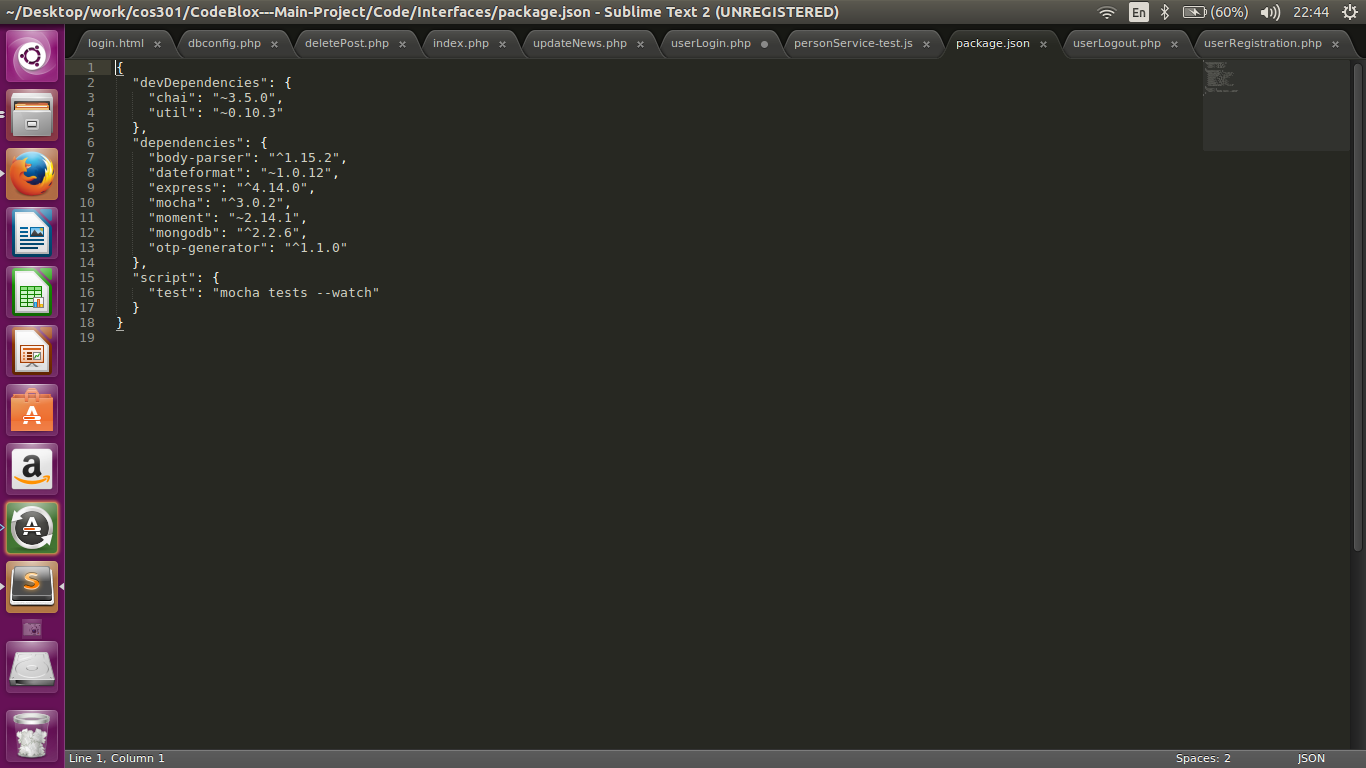
\includegraphics[width=1\textwidth]{./Pictures/3.png}\\[1.5cm] \newline
				
	\section{Conclusions and Recommendations}
	We have gained much insight in terms of testing and its uses. We switched to a testing strategy called Test Driven Development, hereto referred as TTD. With TTD, we are able to write tests without any code written to pass it. This enables the user to write unbiased code because we have no knowledge of the inner code. 
	
	We have also learnt to write tests that test a function in depth. This was achieved by using a special library called chai that is used in conjunction with mocha. It has a vast library of asserts that can be used.
	
	Overall, we are happy with our progress as far as testing is concerned. After completion, if time allows, we wish to carry out a usability test.
				
			
			
			
			
			
		
		
		
		
		
\end{document}
		
		